\begin{frame}
    \frametitle{Git and GitHub}
    \framesubtitle{Getting started with Git}
    \addtocounter{nframe}{1}
    
	\begin{block}{Git command line environment}
		The command line is the only place you can run all Git commands.
    \end{block}

	\begin{block}{GUIs environment}
		GUIs implement only a partial subset of Git functionality for simplicity
    \end{block}
	
\end{frame}

\begin{frame}
	\frametitle{Git and GitHub}
    \framesubtitle{Getting started with Git}
    \addtocounter{nframe}{1}

	\begin{center}
		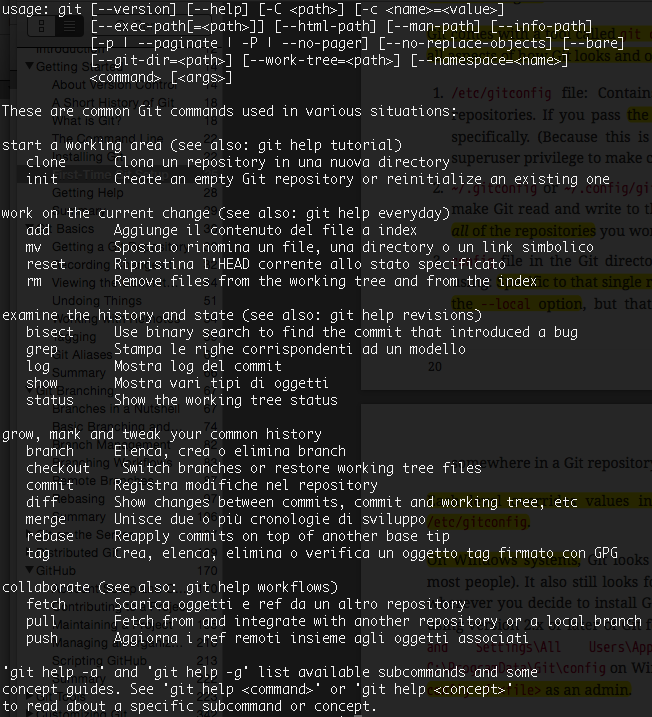
\includegraphics[width=.7\textwidth]{imgs/git-commands.png}
	\end{center}

\end{frame}

\begin{frame}
    \frametitle{Git and GitHub}
    \framesubtitle{Getting started with Git}
    \addtocounter{nframe}{1}
	
	\emph{Git comes with a tool called \textbf{git config} that lets you get and set configuration variables that control all aspects of how Git looks and operates}

	\begin{block}{git config}
		\begin{itemize}
			\item system (all users, all repositories)
			\item global (all repositories, single user)
			\item local (single repository, single user)
		\end{itemize}
    \end{block}

\end{frame}

\begin{frame}
    \frametitle{Git and GitHub}
    \framesubtitle{Getting started with Git}
    \addtocounter{nframe}{1}
	
	\emph{The first thing you should do when you install Git is to set your \textbf{user} name and \textbf{email} address
	}

	\begin{block}{git config}
		\begin{itemize}
			\item \texttt{git config --global user.name "Angelo Mario Del Grosso"}
			\item \texttt{git config --global user.email "angelo.delgrosso@ilc.cnr.it"}
		\end{itemize}
    \end{block}

\end{frame}

\begin{frame}
	\frametitle{Git and GitHub}
    \framesubtitle{Checking Your Settings}
    \addtocounter{nframe}{1}

	\begin{center}
		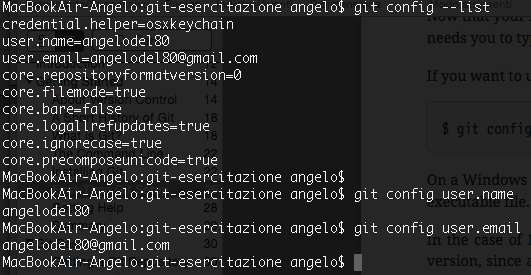
\includegraphics[width=.95\textwidth]{imgs/git-config.png}
	\end{center}

\end{frame}

\begin{frame}
    \frametitle{Git and GitHub}
    \framesubtitle{Getting started with Git}
    \addtocounter{nframe}{1}
	
	\begin{block}{help while using git}
		\begin{itemize}
			\item \texttt{git help <verb>}
			\item \texttt{man git-<verb>}
			\item \texttt{git <verb> --help}
			\item \texttt{git <verb> -h}
		\end{itemize}
    \end{block}

\end{frame}


\begin{frame}
    \frametitle{Git and GitHub}
    \framesubtitle{Getting started with Git}
    \addtocounter{nframe}{1}
	
	\begin{block}{fundamental capabilities}
		\begin{itemize}
			\item configure and initialize a repository
			\item tracking files
			\item stage and commit changes
			\item ignore certain files and file patterns
			\item undo mistakes
			\item browse the history and view changes
			\item push and pull from remote repositories
		\end{itemize}
    \end{block}

\end{frame}

\begin{frame}
    \frametitle{Git and GitHub}
    \framesubtitle{Getting started with Git}
    \addtocounter{nframe}{1}
	
	\begin{block}{git repository}
		\begin{itemize}
			\item local directory that is not under version control, and turn it into a git repository
			\item clone an existing Git repository from elsewhere
		\end{itemize}
    \end{block}

\end{frame}

\begin{frame}
    \frametitle{Git and GitHub}
    \framesubtitle{Getting started with Git}
    \addtocounter{nframe}{1}
	
	\begin{block}{git repository init}
		\begin{itemize}
			\item \texttt{git init}
			\item \texttt{git clone <URL> <DIR>}
		\end{itemize}
    \end{block}

\end{frame}

\begin{frame}
    \frametitle{Git and GitHub}
    \framesubtitle{Getting started with Git}
    \addtocounter{nframe}{1}
	
	\begin{block}{git repository init}
		After \textbf{init} nothing in the project is tracked yet.\\
		Need to begin tracking those files and do an initial commit.
	\end{block}

	\begin{block}{specify the files you want to track}
		\begin{itemize}
			\item \texttt{git add <FILE(S)>}
			\item \texttt{git commit -m "<MESSAGE>"}
		\end{itemize}
	\end{block}
	
	\textit{Git repository with tracked files and an initial commit}
    
\end{frame}

\begin{frame}
    \frametitle{Git and GitHub}
    \framesubtitle{Getting started with Git}
    \addtocounter{nframe}{1}
	
	\begin{block}{git clone repository}
		Every version of every file for the history of the project is pulled down by default when you run \texttt{git clone}
    \end{block}

\end{frame}

\begin{frame}
    \frametitle{Git and GitHub}
    \framesubtitle{Getting started with Git}
    \addtocounter{nframe}{1}
	
	\begin{block}{git repository init}
		Each file in your working directory can be in one of two states
	\end{block}

	\begin{block}{track files}
		\begin{itemize}
			\item tracked
			\item untracked
		\end{itemize}
	\end{block}
	
	\textit{Tracked files are files that were in the last snapshot; they can be \textbf{unmodified}, \textbf{modified}, or \textbf{staged}}
    
\end{frame}

\begin{frame}
	\frametitle{Git and GitHub}
    \framesubtitle{track files}
    \addtocounter{nframe}{1}

	\begin{center}
		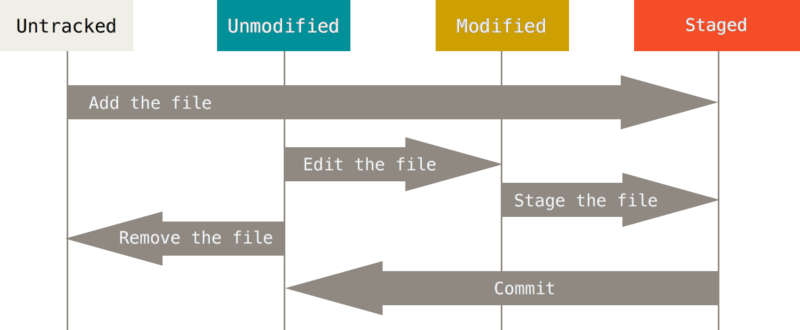
\includegraphics[width=.95\textwidth]{imgs/git-lifecycle-files.png}
	\end{center}

\end{frame}

\begin{frame}
	\frametitle{Git and GitHub}
    \framesubtitle{status files}
    \addtocounter{nframe}{1}

	\textit{To determine which files are in which state: \textbf{the git status command}}

	\begin{center}
		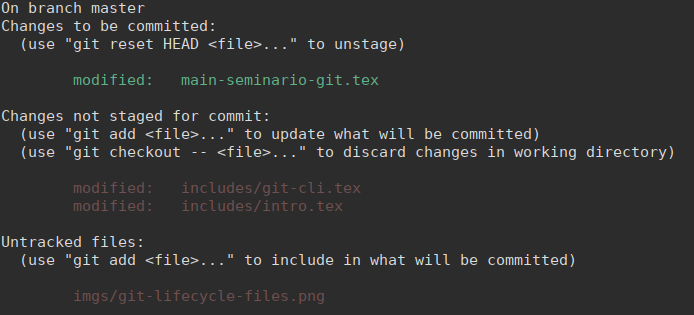
\includegraphics[width=.9\textwidth]{imgs/git-status.png}
	\end{center}

\end{frame}

\begin{frame}
	\frametitle{Git and GitHub}
    \framesubtitle{adding files}
    \addtocounter{nframe}{1}


	\begin{block}{git add}
		In order to begin tracking a new file, you use the \textbf{command git add}
	\end{block}

	\begin{block}{git add}
		file is now \textbf{tracked} and \textbf{staged} to be \textbf{committed}
	\end{block}

	\textit{The git add command \textbf{takes a path name} for either a file or a directory}
	

\end{frame}

\begin{frame}
	\frametitle{Git and GitHub}
    \framesubtitle{adding files}
    \addtocounter{nframe}{1}


	\begin{block}{git add}
		File that is tracked has been modified in the working directory but not yet staged
	\end{block}

	\begin{block}{git add}
		To stage a modified tracked file, you have to run the \textbf{git add command} again.
	\end{block}
	
	\textit{After git add, the files are staged and will go into your next commit}	

\end{frame}

\begin{frame}
	\frametitle{Git and GitHub}
    \framesubtitle{adding files}
    \addtocounter{nframe}{1}


	\begin{block}{git add}
		If you modify a file after you run git add, you have to run git add again to stage the latest version of the file
	\end{block}

	\begin{center}
		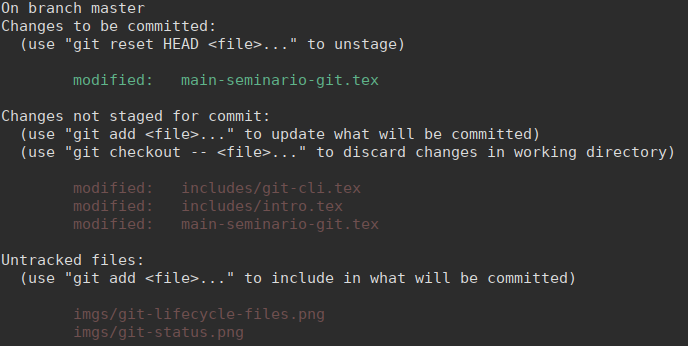
\includegraphics[width=.9\textwidth]{imgs/git-add-modify.png}
	\end{center}

\end{frame}

\begin{frame}
	\frametitle{Git and GitHub}
    \framesubtitle{ignoring files}
    \addtocounter{nframe}{1}


	\begin{block}{.gitignore file}
		If you’ll have a class of files that you don’t want to track
	\end{block}

	\begin{block}{.gitignore file}
		you can create a file listing patterns to match them named \textbf{.gitignore}.
	\end{block}

\end{frame}

\begin{frame}
	\frametitle{Git and GitHub}
    \framesubtitle{ignoring files}
    \addtocounter{nframe}{1}

	\begin{center}
		\texttt{more .gitignore}
	\end{center}
	
	\begin{center}
		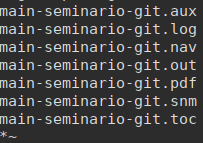
\includegraphics[width=.7\textwidth]{imgs/gitignore.png}
	\end{center}

\end{frame}

\begin{frame}
	\frametitle{Git and GitHub}
    \framesubtitle{viewing files}
    \addtocounter{nframe}{1}

	\begin{block}{git diff}
		know exactly what you changed, not just which files were changed\\
		by using the \textbf{git diff command}
	\end{block}

	\begin{block}{git diff}
		\begin{itemize}
			\item What have you changed but not yet staged (\texttt{git diff})
			\item what have you staged that you are about to commit (\texttt{git diff --staged})
		\end{itemize}
	
	\end{block}

\end{frame}

\begin{frame}
	\frametitle{Git and GitHub}
    \framesubtitle{viewing files}
    \addtocounter{nframe}{1}
	
	\begin{center}
		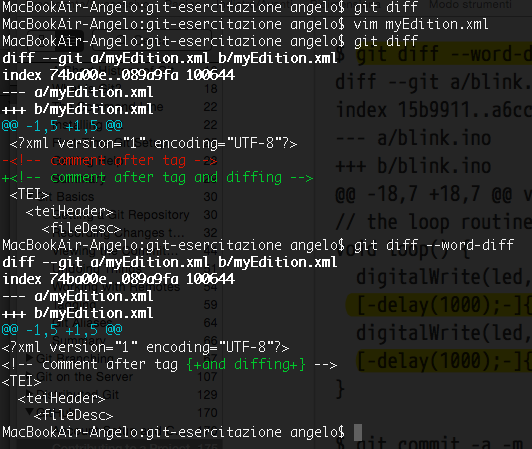
\includegraphics[width=.8\textwidth]{imgs/Diffing-line-word.png}
	\end{center}

\end{frame}

\begin{frame}
	\frametitle{Git and GitHub}
    \framesubtitle{committing files}
    \addtocounter{nframe}{1}

	\begin{block}{git commit}
		Any files you have created or modified that you haven’t run git add on since you edited them — won’t go into the commit.
	\end{block}

	\begin{block}{git commit}
		\begin{itemize}
			\item the simplest way to commit is to type (\texttt{git commit})
			\item type your commit message inline  (\texttt{git commit -m "message"})
		\end{itemize}
	
	\end{block}

\end{frame}

\begin{frame}
	\frametitle{Git and GitHub}
    \framesubtitle{committing files}
    \addtocounter{nframe}{1}

	\begin{block}{git commit}
		Every time you perform a commit, you’re recording a snapshot of your project that you can revert to or compare to later.
	\end{block}

	\begin{center}
		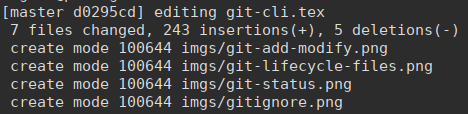
\includegraphics[width=.8\textwidth]{imgs/git-commit.png}
	\end{center}

\end{frame}

\begin{frame}
	\frametitle{Git and GitHub}
    \framesubtitle{removing files}
    \addtocounter{nframe}{1}

	\begin{block}{git rm}
		To remove a file from git, you have to remove it from your tracked files
	\end{block}

	\begin{block}{git rm}
		\begin{itemize}
			\item \texttt{git rm <FILE>}
			\item \texttt{git rm -f <FILE>}
			\item \texttt{git rm --cached <FILE>}
		\end{itemize}
	
	\end{block}

\end{frame}

\begin{frame}
	\frametitle{Git and GitHub}
    \framesubtitle{moving files}
    \addtocounter{nframe}{1}

	\begin{block}{git mv}
		If you rename a file in Git, no metadata is stored in Git that tells it you renamed the file
	\end{block}

	\begin{block}{git mv}
		\begin{itemize}
			\item \texttt{git mv <FILE-FROM> <FILE-TO>}
		\end{itemize}
	\end{block}

\end{frame}

\begin{frame}
	\frametitle{Git and GitHub}
    \framesubtitle{moving files}
    \addtocounter{nframe}{1}

	\begin{block}{git mv}
		\begin{itemize}
			\item \texttt{mv <FILE-FROM> <FILE-TO>}
			\item \texttt{git rm <FILE-FROM>}
			\item \texttt{git add <FILE-TO>}
		\end{itemize}
	\end{block}
\end{frame}

\begin{frame}
	\frametitle{Git and GitHub}
    \framesubtitle{History of commits}
    \addtocounter{nframe}{1}

	\begin{block}{git log}
		\textbf{git log} lists the commits made in that repository in reverse chronological order, each commit with its checksum hash string, author’s name and email, date, the commit message.
	\end{block}

	\begin{block}{git log}
		\begin{itemize}
			\item \texttt{git log <options>}
		\end{itemize}
	\end{block}

\end{frame}

\begin{frame}
	\frametitle{Git and GitHub}
    \framesubtitle{History of commits}
    \addtocounter{nframe}{1}

	\begin{block}{git log}
		if you want to see some abbreviated stats for each commit, you can use \textbf{the --stat option}
	\end{block}

	\begin{block}{git log}
		\begin{itemize}
			\item \texttt{git log --stat}
		\end{itemize}
	\end{block}

\end{frame}

\begin{frame}
	\frametitle{Git and GitHub}
    \framesubtitle{History of commits}
    \addtocounter{nframe}{1}

	
		\begin{center}
			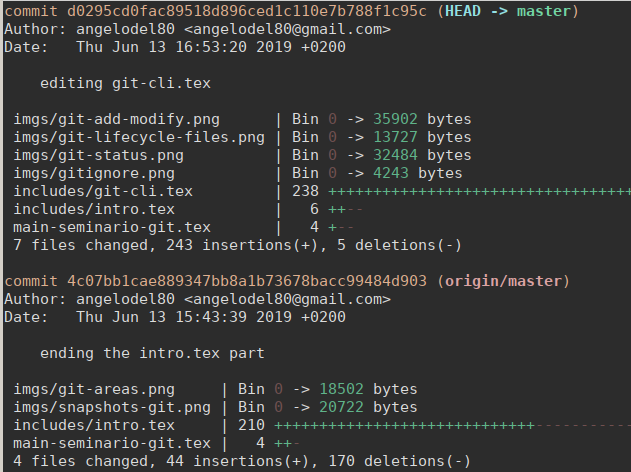
\includegraphics[width=.8\textwidth]{imgs/git-log-stats.png}
		\end{center}
	
\end{frame}

\begin{frame}
	\frametitle{Git and GitHub}
    \framesubtitle{History of commits}
    \addtocounter{nframe}{1}

	\begin{block}{git log options}
		\begin{center}
			%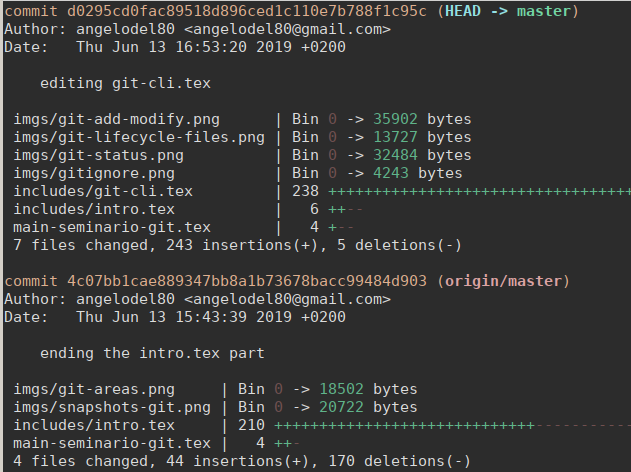
\includegraphics[width=.9\textwidth]{imgs/git-log-stats.png}
			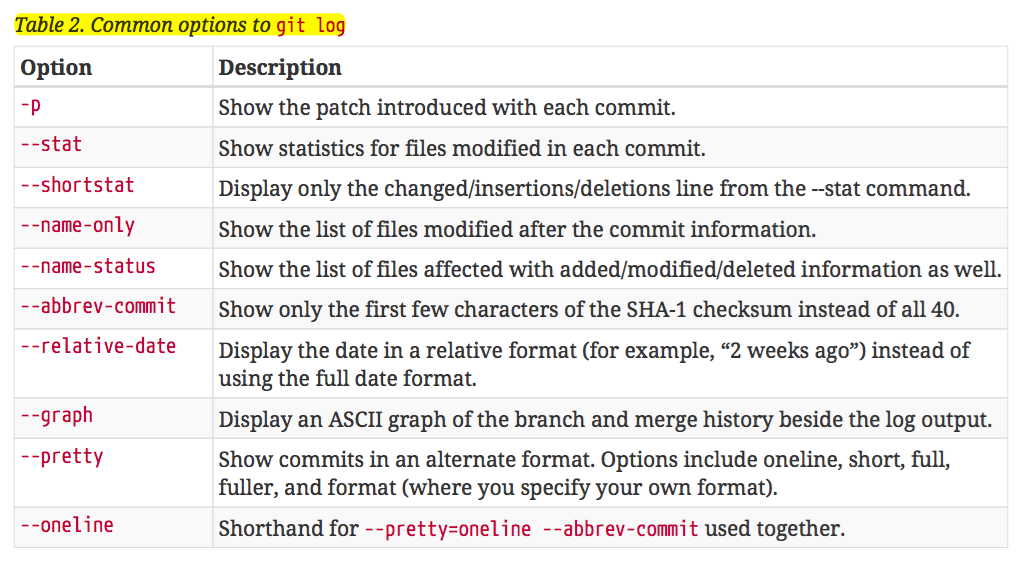
\includegraphics[width=.95\textwidth]{imgs/git-log-options.png}
		\end{center}
	\end{block}

\end{frame}

\begin{frame}
	\frametitle{Git and GitHub}
    \framesubtitle{git log --pretty}
    \addtocounter{nframe}{1}


		\begin{center}
			%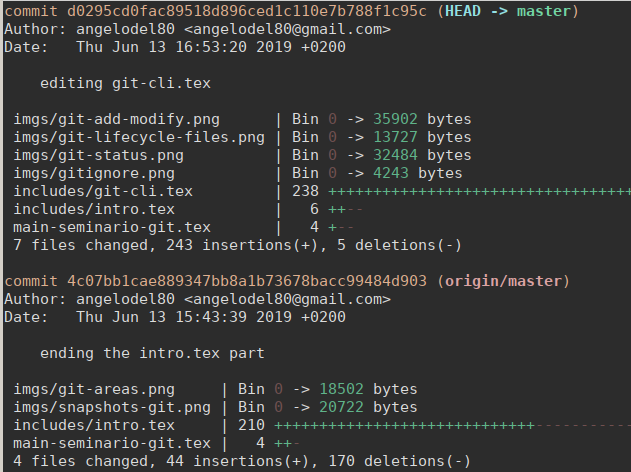
\includegraphics[width=.9\textwidth]{imgs/git-log-stats.png}
			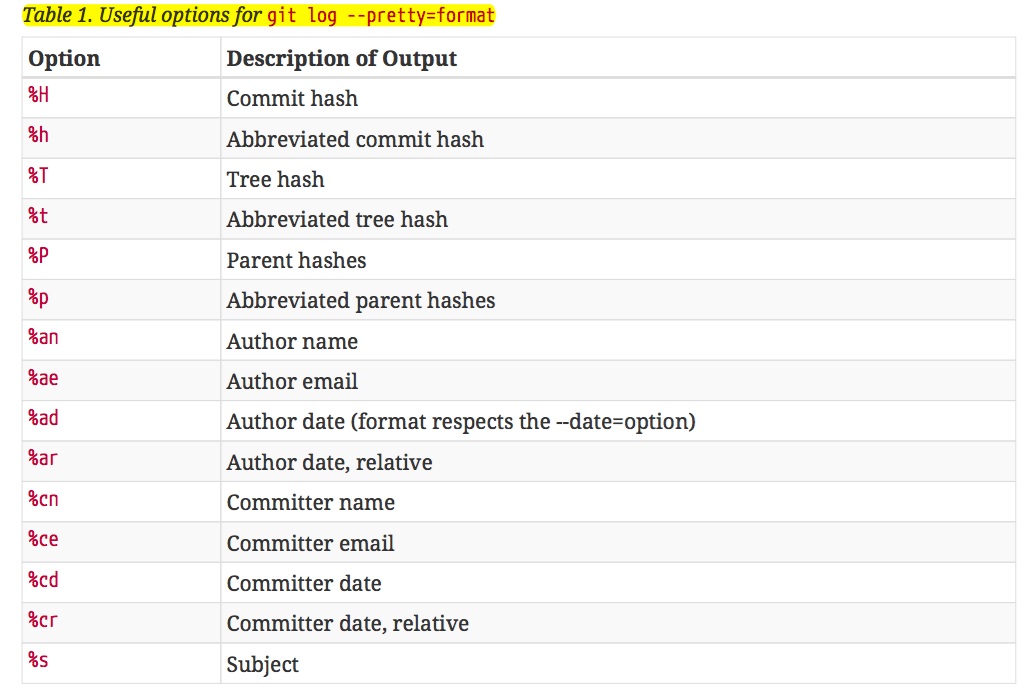
\includegraphics[width=.9\textwidth]{imgs/git-log-pretty.png}
		\end{center}

\end{frame}

\begin{frame}
	\frametitle{Git and GitHub}
    \framesubtitle{History of commits}
    \addtocounter{nframe}{1}

	\begin{block}{git log limit options}
		\begin{center}
			%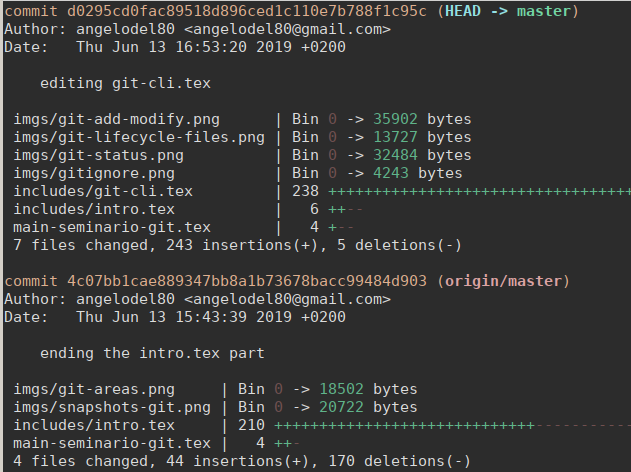
\includegraphics[width=.9\textwidth]{imgs/git-log-stats.png}
			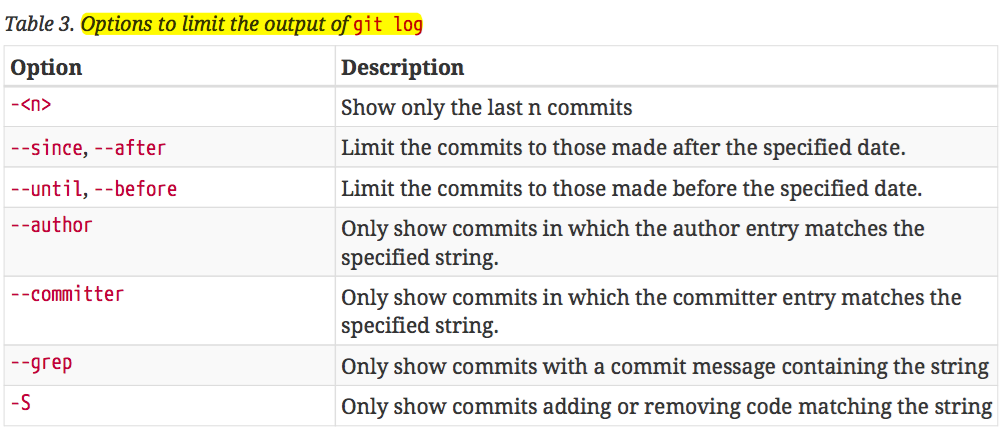
\includegraphics[width=.95\textwidth]{imgs/git-log-limits.png}
		\end{center}
	\end{block}

\end{frame}

\begin{frame}
	\frametitle{Git and GitHub}
    \framesubtitle{History of commits}
    \addtocounter{nframe}{1}

	\texttt{git log --pretty="\%h: \%an -- \%s" --no-merges}
	\begin{block}{git log --pretty}
		\begin{center}
			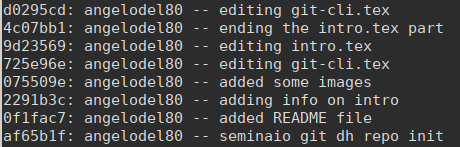
\includegraphics[width=.9\textwidth]{imgs/git-log-out.png}
		\end{center}
	\end{block}

\end{frame}

\begin{frame}
	\frametitle{Git and GitHub}
    \framesubtitle{Undoing things}
    \addtocounter{nframe}{1}

	\begin{block}{amend option}
		If you commit too early and possibly forget to add some files, make the additional changes you forgot, stage them, and \textbf{commit again using the --amend option}.
		\\ You end up with a single commit — the \textit{second commit replaces the first one}.
	\end{block}

	\begin{block}{git log}
		\begin{itemize}
			\item \texttt{git commit --amend [-m "MESSAGE"]}
		\end{itemize}
	\end{block}

\end{frame}

\begin{frame}
	\frametitle{Git and GitHub}
    \framesubtitle{Undoing things}
    \addtocounter{nframe}{1}

	\begin{block}{unstage and discard changes}
		How can you unstage a file or revert it back to what it looked like when you last committed.
	\end{block}

	\begin{block}{git reset and checkout}
		\begin{itemize}
			\item \texttt{git reset HEAD <FILE>} (unstage file)
			\item \texttt{git checkout -- <FILE>} (discard changes)
		\end{itemize}
	\end{block}

\end{frame}

\begin{frame}
	\frametitle{Git and GitHub}
    \framesubtitle{Working with Remotes}
    \addtocounter{nframe}{1}

	\begin{block}{Remote Repositories}
		Remote repositories are versions of your project that are hosted on the Internet
	\end{block}

	\begin{block}{Remote Repositories}
		Collaborating with others involves managing remote repositories. \\
		This entails \textbf{pushing} and \textbf{pulling} data to and from remote repositories when you need to share data.
	\end{block}

\end{frame}

\begin{frame}
	\frametitle{Git and GitHub}
    \framesubtitle{Working with Remotes}
    \addtocounter{nframe}{1}

	\begin{block}{capabilities}
		\begin{itemize}
			\item add remote repositories
			\item remove remotes
			\item manage various remote branches
			\item define them as being tracked or not
			\item pushing, pulling and fetching operations
		\end{itemize}
	\end{block}

\end{frame}

\begin{frame}
	\frametitle{Git and GitHub}
    \framesubtitle{Working with Remotes}
    \addtocounter{nframe}{1}

	\begin{block}{remote repositories}
		To see which remote servers you have configured, you can run the \textbf{git remote command}
	\end{block}

	\begin{block}{git remote}
		\begin{itemize}
			\item \texttt{git remote}
			\item \texttt{git remote -v}
		\end{itemize}
	\end{block}

\end{frame}

\begin{frame}
	\frametitle{Git and GitHub}
    \framesubtitle{Working with Remotes}
    \addtocounter{nframe}{1}

	\begin{block}{remote repositories}
		To add a new remote Git repository as a shortname you can reference easily, run \textbf{git remote add <shortname> <url>}:
	\end{block}

	\begin{block}{git remote}
		\begin{itemize}
			\item \texttt{git remote add upstream-edition https://github.com/angelodel80/myEditon}
		\end{itemize}
	\end{block}

	\textit{If you clone a repository, the command automatically adds that remote repository under the name “origin”}

\end{frame}

\begin{frame}
	\frametitle{Git and GitHub}
    \framesubtitle{Working with Remotes}
    \addtocounter{nframe}{1}

	\begin{block}{remote repositories}
		to get data from your remote projects, you can run the \textbf{git fetch command}. \\
		It’s important to note that the git fetch command only downloads the data to your local repository — it doesn't automatically merge it with any of your work or modify what you’re currently working on.
	\end{block}

	\begin{block}{git remote}
		\begin{itemize}
			\item \texttt{git fetch <remote>}
		\end{itemize}
	\end{block}

\end{frame}

\begin{frame}
	\frametitle{Git and GitHub}
    \framesubtitle{Working with Remotes}
    \addtocounter{nframe}{1}

	\begin{block}{remote repositories}
		When you have your project at a point that you want to share, you have to \textbf{push it upstream}. This pushes any commits you’ve done back up to the server if you have write access and if nobody has pushed in the meantime.
	\end{block}

	\begin{block}{git remote}
		\begin{itemize}
			\item \texttt{git push <remote> <branch>}
		\end{itemize}
	\end{block}

\end{frame}

\begin{frame}
	\frametitle{Git and GitHub}
    \framesubtitle{Working with Remotes}
    \addtocounter{nframe}{1}


	\begin{block}{git remote}
		\begin{itemize}
			\item \texttt{git remote show <remote>}
		\end{itemize}
	\end{block}


	\begin{block}{remote repositories}
		\begin{center}
			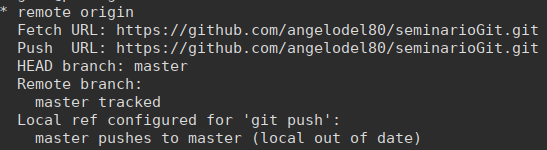
\includegraphics[width=.9\textwidth]{imgs/git-remote-show}
		\end{center}
	\end{block}

\end{frame}

\begin{frame}
	\frametitle{Git and GitHub}
    \framesubtitle{Working with Remotes}
    \addtocounter{nframe}{1}

	\begin{block}{remote repositories}
		You can run \textbf{git remote rename} to change a remote’s shortname, if you want to remove a remote repository you can either use \textbf{git remote remove} command or \textbf{git remote rm} command. 

	\end{block}

	\begin{block}{git remote}
		\begin{itemize}
			\item \texttt{git remote rename original upstream-edition}
			\item \texttt{git remote remove upstream-edition}
		\end{itemize}
	\end{block}

\end{frame}

\begin{frame}
	\frametitle{Git and GitHub}
    \framesubtitle{Tagging}
    \addtocounter{nframe}{1}

	\begin{block}{tag specific points}
		Git has the ability to \textbf{tag specific points} in a \textit{repository's history} as being important, e.g. mark release points. Git supports two types of tags: lightweight and annotated.
	\end{block}

\end{frame}

\begin{frame}
	\frametitle{Git and GitHub}
    \framesubtitle{Tagging}
    \addtocounter{nframe}{1}

	\begin{block}{git tag}
		\begin{itemize}
			\item \texttt{git tag [-l] [--list] <PATTERN>} (list tags)
			\item \texttt{git tag -a <TAG-NAME> -m "MESSAGGIO" } (create an annotated tag)
			\item \texttt{git show <TAG-NAME>} (show the tag data)
			\item \texttt{git push <REMOTE> <TAG-NAME>} (push tag)
			\item \texttt{git tag -d  <TAG-NAME>} (delate locally)
			\item \texttt{git push <REMOTE> --delete <TAG-NAME>} (delate remotelly)
		\end{itemize}
	\end{block}

\end{frame}

\begin{frame}
	\frametitle{Git and GitHub}
    \framesubtitle{Tagging}
    \addtocounter{nframe}{1}

	\begin{block}{tag specific points}
		If you want to view the versions of files a tag is pointing to, you can do a git checkout of that tag.\\
		This puts your repository in “detached HEAD” state, which has some ill side effects
	\end{block}

	\begin{block}{git tag}
		\begin{itemize}
			\item \texttt{git checkout <TAG-NAME>} (View the files in tag version)
		\end{itemize}
	\end{block}
\end{frame}
